\documentclass[12pt]{article}
\usepackage[utf8]{inputenc}
\usepackage{polski}
\usepackage[a4paper, left=2.0cm, right=2.0cm, top=2.0cm, bottom=2.0cm]{geometry}
\usepackage{graphicx}
\usepackage{multicol}
\usepackage{hyperref}


\title{PIISW, W08, IO, 2020/2021, semestr letni\\Lista zadań nr 3: Tworzenie i testowanie backendu: serwisy RESTowe}
\author{Adam Puchalski\\ \small adam.puchalski@pwr.edu.pl}

\begin{document}
    \maketitle

    \section*{Zasady Pracy}
    \begin{itemize}
        \item Rozwiązania zadań z~tej listy muszą znaleźć się w~prywatnym repozytorium na \texttt{github.com} (może to być to samo repozytorium, które założono w~ramach prac nad listą nr~2).
        \item Prowadzący zajęcia musi mieć uprawnienia do odczytu i~zapisu do tego repozytorium.
        \item Zadanie \ref{exc:spring_rest} jest obowiązkowe. W~razie jego braku dalsza częsc listy nie bedzie sprawdzana.
    \end{itemize}

\section*{Wprowadzenie}
\begin{itemize}
        \item  W~zadaniu \ref{exc:spring_rest} trzeba zaimplementować uproszczoną wersję reverse-proxy. Jako takie reverse-proxy nie ma żadnej logiki biznesowej i~służy jedynie jako pośrednik odbierając requesty i~przekazując je dalej. Reverse-proxy ukrywa architekturę systemów po stronie odbiorcy przed nadawcą, on (nadawca) niezależnie od rodzaju requestu cały czas rozmawia z~jednym systemem (proxy).
        \item Kolejne zadania uzupełniają implementację serwera o~testy Junitowe (jednostkowe bądź integracyjne), obsługę wyjątków oraz typowe testy integracyjne.
        \item Ostatnie zadanie polega na podłączeniu CI do repozytorium z~zadaniem i~doprowadzenie stanu builda do zieleni.
\end{itemize}

    \section*{Oceny}
    \begin{tabular}{|l|c|c|c|c|c|c|}
        \hline
        Punkty: & $<7$ & $7-8$ & $9-10$ & $11-12$ & $13-14$ & 15\\
        \hline
        Ocena:  & $2,0$ & $3,0$ & $3,5$ & $4,0$ & $4,5$ & $5,0$\\
        \hline
    \end{tabular}

    \section*{Zadania}
    \begin{enumerate}
        \item\label{exc:spring_rest}
            (4 pkt) Reverse-Proxy - zadanie podstawowe.\\
            W~ramach ćwiczeń do zaimplementowania jest szary element z~rysunku \ref{fig:lista_3_proxy}. Posiada on interfejs RESTowy wejściowy i~wyjściowy.
            \begin{itemize}
                \item Interfejs wejściowy przyjmuje request od nadawcy i~w~zależnosci od jego typu przekazuje do odpowiedniego adresata (System 1-3). Gdy adresat przetworzy request, jego odpowiedź jest zwracana do nadawcy.
                \item Ponieważ systemy zewnętrzne nie istnieją, należy je zamockować z~użyciem dowolnego narzędzia (wiremock, json-server, ...)
                \item Konfiguracja adresów systemów zewnętrznych powinna znaleźć się w~pliku \texttt{applica\-tion.pro\-per\-ties} w~formie np. \texttt{destination.get=localhost:8899}
            \end{itemize}
            
	\begin{figure}[hb]
        \centering
        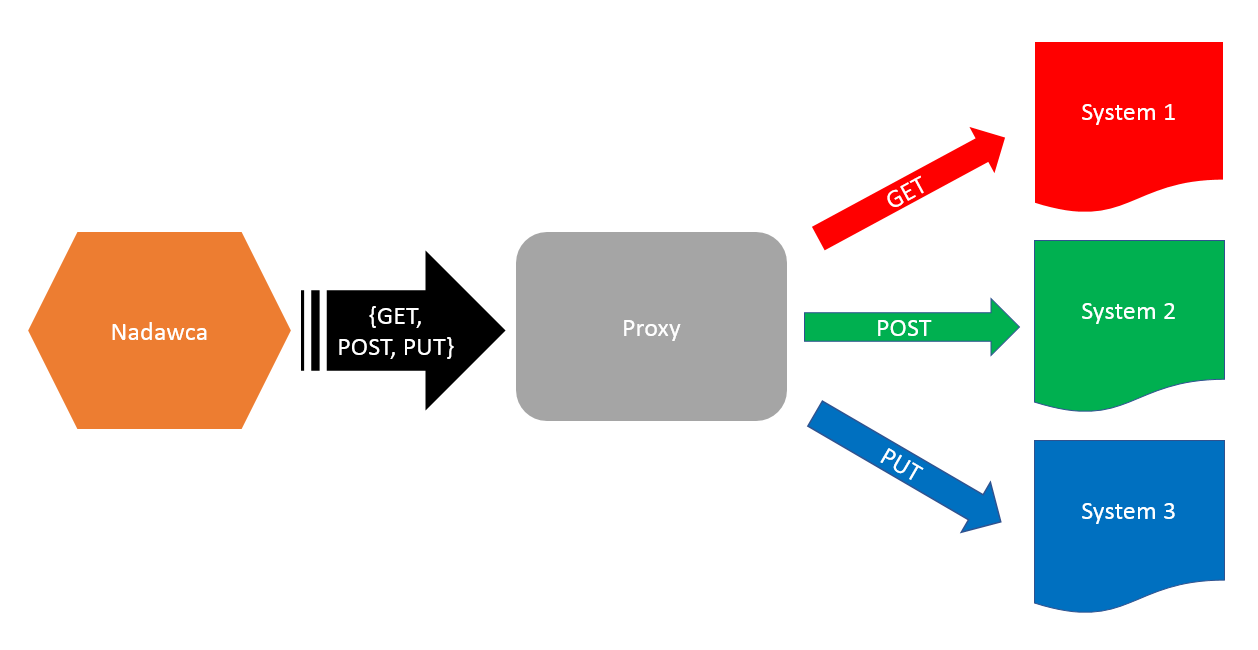
\includegraphics[width=\textwidth]{lista_3_proxy}
        \caption{Diagram obrazujący sposób działania reverse proxy implementowanego w ramach zadania \ref{exc:spring_rest}.}
        \label{fig:lista_3_proxy}
    \end{figure}

    \textbf{Wskazówka:} Zalecane jest rozpoczęcie od nowego springbootowego projektu z~modułem Web (zob. \url{https://start.spring.io}) oraz zaznajomienie sie z~\texttt{RestController} i~\texttt{RestTemplate}.

        \item\label{exc:spring_rest_test}
            (3 pkt) Testowanie automatyczne.\\
W~ramach ćwiczenia trzeba stworzone w~zadaniu \ref{exc:spring_rest} reverse-proxy pokryć testami automatycznymi.
\begin{itemize}
        \item Dla każdego rodzaju requestu powinien zostać napisany co najmniej jeden test automatyczny.
        \item Jesli rodzaj testu tego wymaga, zależnosć (czyli obecność systemu będącego na końcu testowanego interfejsu) musi być uruchamiana przez sam test, a~nie przez użytkownika zanim testy zostaną uruchomione
\end{itemize}

\textbf{Wskazówka:} Zalecane jest zaznajomienie się z~\texttt{TestRestTemplate} oraz np. \texttt{Wiremock} i jego wsparciem dla JUnitów.

        \item\label{exc:spring_exception_handling}
            (2 pkt) Obsługa wyjątków.\\
Reverse-proxy nie jest w stanie interpretować błędów jakie mogą się przytrafić podczas komunikacji systemami zewnętrznymi, musi więc komunikaty o~błędach odpowiednio przekazywać dalej.
\begin{itemize}
        \item Do obsługi wyjątków należy użyć \texttt{ControllerAdvice}.
        \item W~zależnosci od implementacji testy automatyczne powinny być rozszerzone o~przypadki sprawdzające sytuacje w~których system musi obsługiwać wyjątki.
\end{itemize}

        \item\label{exc:postman}
            (3 pkt) Testowanie integracyjne.\\
\begin{itemize}
        \item Do testowania integracyjnego zalecane jest użycie aplikacji \texttt{Postman}. Przyklady odnosnie pisania testów api z użyciem tego narzędzia są tutaj: \\\url{http://blog.getpostman.com/2014/03/07/writing-automated-tests-for-apis-using-postman/}
        \item Dla każdego rodzaju requestu powinny zostać napisane conajmniej dwa test integracyjne (1 pozytywny i 1 negatywny).
\end{itemize}

        \item\label{exc:travis}
            (3 pkt) CircleCI.\\
W~ramach tego ćwiczenia trzeba do serwisu \texttt{circleci.com} podłączyć swoje repozytorium z~zaimplementowanym reverse-proxy i~doprowadzić build do zieleni - aby się kompilował oraz żeby wszystkie testy były "zielone".

    \end{enumerate}
\end{document}

